
\documentclass[twocolumn,10pt]{article}
\title{Constructing triangles}
\setlength{\columnsep}{20pt} 
\usepackage{amsmath,hyperref,cancel,graphicx}
 \def\shrinkfactor{0.45}
 \usepackage[margin=1.5cm]{geometry}
\usepackage[usenames,dvipsnames]{color}
 
 \newcommand{\blue}[1]{{\color{Blue}#1}} 
 \newcommand{\purple}[1]{{\color{Purple}#1}} 
 \newcommand{\red}[1]{{\color{Red}#1}} 
 \newcommand{\green}[1]{{\color{Green}#1}} 
 \newcommand{\gray}[1]{{\color{Gray}#1}} 
  \newcommand{\pink}[1]{{\color{Magenta}#1}}   






\begin{document}
\maketitle



\section{\href{https://www.khanacademy.org/devadmin/content/items/x0a2c8d4a7e3a85b9}{x0a2c8d4a7e3a85b9}}

\noindent
**How many triangles can be drawn where we know two angles and the side length between the two angles?**

\paragraph{Ans} 

None

\fbox{ Only one

}

 More than one



\paragraph{Hint 1}Let's draw an example of a triangle where the side length is known between two angles. Let's look at when a side of length $\blue4$ is between a pair of $\blue{75^\circ}$ angles.

\paragraph{Hint 2}The other two sides can be drawn at $\blue{75^\circ}$ angles  and are equal in length. The sides meet at a $\blue{30^\circ}$ angle to complete the triangle. 


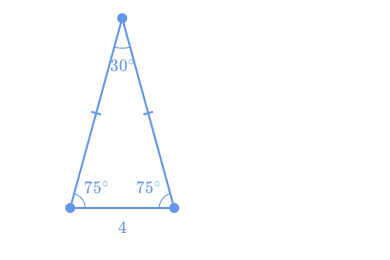
\includegraphics[scale=\shrinkfactor]{figures/8664b06c420b8bf33711310103a6963e0f2cc7f1.png}

This triangle is unique, meaning no other triangle exists with the same shape and size.

\paragraph{Hint 3}When the side length is known between two known angles, only one triangle can be drawn.



\medskip
\noindent
\textbf{Tags:} {\footnotesize Constructing triangles, CC.7.G.A.2}\\
\textbf{Version:} 4a925246.. 2013-10-21
\smallskip\hrule





\section{\href{https://www.khanacademy.org/devadmin/content/items/x18341f6f8d24d96e}{x18341f6f8d24d96e}}

\noindent
**How many triangles can be drawn with side lengths $9$, $12$ and $15$?**



\paragraph{Ans} 

None

\fbox{ Only one

}

 More than one



\paragraph{Hint 1}A triangle is a plane figure with three straight sides and three angles. Can we satisfy the definition given the conditions? Let's try to draw a triangle given the conditions.

\paragraph{Hint 2}In general, any side of a triangle is always shorter than the sum of the other two sides:

\begin{align*}\phantom{over}\blue{15} &<\blue{9}+\blue{12} \\\phantom{over}\blue{12}&<
 \blue{9}+\blue{15} \\\phantom{over}\blue{9}&<
 \blue{12}+\blue{15} \\\end{align*}

We can create a triangle with a unique size and shape.


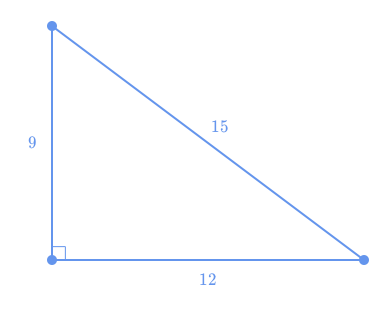
\includegraphics[scale=\shrinkfactor]{figures/9e3335e4646b2e59f3ceb8860cd9099de97f22b0.png}

\paragraph{Hint 3}Given the conditions, only one triangle can be drawn.



\medskip
\noindent
\textbf{Tags:} {\footnotesize Constructing triangles, CC.7.G.A.2}\\
\textbf{Version:} 49159f6f.. 2013-10-21
\smallskip\hrule





\section{\href{https://www.khanacademy.org/devadmin/content/items/x1afa3df30210708e}{x1afa3df30210708e}}

\noindent
**Draw a right triangle with side lengths $5a$,  $12a$ and $13a$, where $a$ is any positive number.**

**Is there a unique triangle that satisfies the given conditions?**  
[[? interactive-graph 1]]

\paragraph{Ans} 

Yes

\fbox{ No

}

 

\paragraph{Hint 1}Let�s start by choosing a value for $\pink{a}$ where $\pink{a}$ is any positive number, then we can draw a right triangle with side lengths $\purple5\pink{a}$, $\purple{12}\pink{a}$ and $\purple{13}\pink{a}$.

\paragraph{Hint 2}Choosing $\pink{a}=\pink{1}$, we can draw a right triangle with side lengths  $\blue{5}$, $\blue{12}$ and $\blue{13}$.


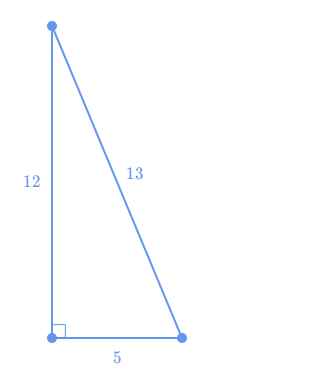
\includegraphics[scale=\shrinkfactor]{figures/6d298ed14c507f692b6d88792d963d7008b9847a.png}

\paragraph{Hint 3}Choosing $\pink{a}=\pink{0.5}$, we can draw a right triangle with side lengths $\blue{2.5}$, $\blue{6}$ and $\blue{6.5}$.   

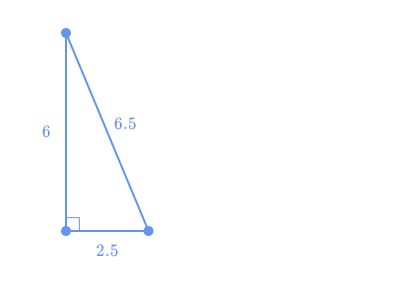
\includegraphics[scale=\shrinkfactor]{figures/463955e595c31361c49d853aea12289b0f5f7779.png} 


\paragraph{Hint 4}The triangle is not unique. We can let $\pink{a}$ be any positive number and draw many triangles with the same shape but different sizes.


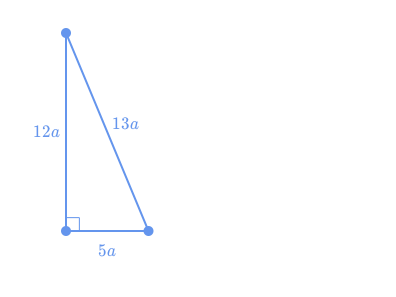
\includegraphics[scale=\shrinkfactor]{figures/28bab6f73b266fa0cb6392a48f06caca532f0cd2.png}



\medskip
\noindent
\textbf{Tags:} {\footnotesize Constructing triangles, CC.7.G.A.2}\\
\textbf{Version:} f00b6980.. 2013-10-21
\smallskip\hrule





\section{\href{https://www.khanacademy.org/devadmin/content/items/x1c875467bbf94500}{x1c875467bbf94500}}

\noindent
**Draw a triangle with side length $4$ between two $70^\circ$ angles.** 

**Is there a unique triangle that satisfies the given conditions?**
[[? interactive-graph 1]]

\paragraph{Ans} 

\fbox{ Yes

}

 No



\paragraph{Hint 1}Let�s start by drawing the side whose length  is $\blue{4}$.

\paragraph{Hint 2}From the side $\blue4$, let�s draw two $\blue{70^\circ}$ angles. Since we have two equal angles, we have an isosceles triangle. An isosceles triangle has at least two sides equal in length. 

Since we have two $\blue{70^\circ}$ angles, the third angle must be $\green{40^\circ}$. The sum of three angles in a triangle will always be $\pink{180^\circ}$.

\paragraph{Hint 3}We know the measure of two angles and the length of the side between the angles, so we can draw only one triangle.

\paragraph{Hint 4}The triangle is unique.


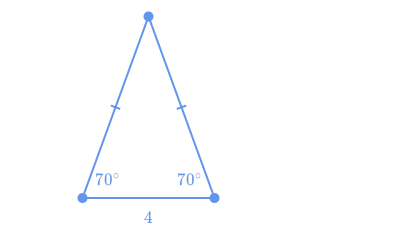
\includegraphics[scale=\shrinkfactor]{figures/42e1efd00be59b64d19c796b09c66213066bd2fa.png}



\medskip
\noindent
\textbf{Tags:} {\footnotesize Constructing triangles, CC.7.G.A.2}\\
\textbf{Version:} 7647d185.. 2013-10-21
\smallskip\hrule





\section{\href{https://www.khanacademy.org/devadmin/content/items/x1da87b180aca0e3d}{x1da87b180aca0e3d}}

\noindent
**How many triangles can be drawn which have side lengths of $5$ and $10$?**

\paragraph{Ans} 

None

Only one

\fbox{ More than one

}

 

\paragraph{Hint 1}We do not know the length of the third side so we are free to choose any length. Thus, we cannot create a unique triangle with only two side lengths.

\paragraph{Hint 2}We can  draw many triangles with side lengths $\blue5$ and $\blue{10}$.


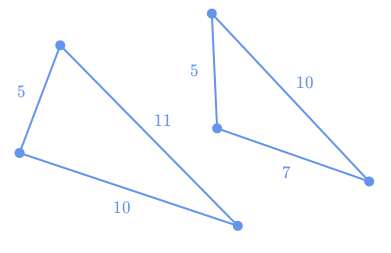
\includegraphics[scale=\shrinkfactor]{figures/fe9bb66c73daee381242a48159a578e8b78ac0fb.png}

\paragraph{Hint 3}If we only know two side lengths, more than one triangle can be drawn.



\medskip
\noindent
\textbf{Tags:} {\footnotesize Constructing triangles, CC.7.G.A.2}\\
\textbf{Version:} d74ae956.. 2013-10-21
\smallskip\hrule





\section{\href{https://www.khanacademy.org/devadmin/content/items/x25470998d7b41ee4}{x25470998d7b41ee4}}

\noindent
**How many triangles can be drawn which have two $45^\circ$ angles and two sides of length $2$?**

\paragraph{Ans} 

None

\fbox{ Only one

}

 More than one



\paragraph{Hint 1}A triangle is a plane figure with three straight sides and three angles. The three angles always add up to $\pink{180^\circ}$. 

Since we have two $\blue{45^\circ}$ angles, the third angle is $\blue{90^\circ}$: 

\begin{align*}\
 &= \pink{180^\circ}-2\cdot\blue{45^\circ} \\
 &= \blue{90^\circ} \end{align*}

Let's draw a right triangle. 

\paragraph{Hint 2}We can draw a right triangle and make two of its sides of length $\blue{2}$. The sides with length $\blue{2}$ must be between the $\blue{45^\circ}$ and $\blue{90^\circ}$ angles.


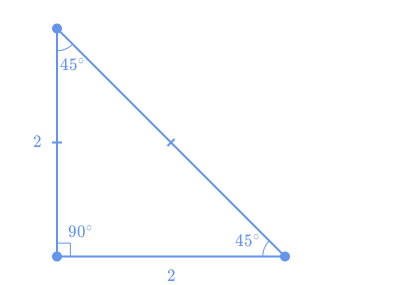
\includegraphics[scale=\shrinkfactor]{figures/50ab52075216ec1ebe030aa80de8615558c71846.png}

This triangle is unique, meaning no other triangle exists with exactly the same shape and size.

\paragraph{Hint 3}Given the conditions, only one triangle can be drawn.



\medskip
\noindent
\textbf{Tags:} {\footnotesize Constructing triangles, CC.7.G.A.2}\\
\textbf{Version:} 2c26d431.. 2013-10-21
\smallskip\hrule





\section{\href{https://www.khanacademy.org/devadmin/content/items/x2bce84b97313fd2b}{x2bce84b97313fd2b}}

\noindent
**Draw a triangle with two angles $31^\circ$ and $90^\circ$ where side length $3$ is *not* between the two angles $31^\circ$ and $90^\circ$.**

**Is there a unique triangle that satisfies the given conditions?**
[[? interactive-graph 1]]

\paragraph{Ans} 

\fbox{ Yes

}

 No



\paragraph{Hint 1}Let�s start by drawing a right angle which is $\blue{90^\circ}$. 

Then, let's draw the side of length $\blue3$ next to the right angle, so our base is length $\blue3$.

\paragraph{Hint 2}The length of $\blue3$ is $\red{\text{not}}$ between two angles $\blue{31^\circ}$ and $\blue{90^\circ}$. 

Since we drew the side of length $\blue3$ next to the right angle, the $\blue{31^\circ}$ angle must be *opposite* the side of length $\blue3$ .

\paragraph{Hint 3}We know the measure of two angles and the length of one side not between the angles, so we can draw only one triangle.

\paragraph{Hint 4}The triangle is unique.


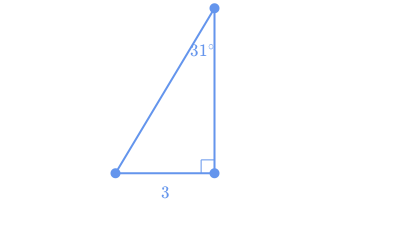
\includegraphics[scale=\shrinkfactor]{figures/48773248b446b970cdf6c2fa7664c3fa8890378a.png}



\medskip
\noindent
\textbf{Tags:} {\footnotesize Constructing triangles, CC.7.G.A.2}\\
\textbf{Version:} 4c8a5b03.. 2013-10-21
\smallskip\hrule





\section{\href{https://www.khanacademy.org/devadmin/content/items/x31c216ff88dad8e7}{x31c216ff88dad8e7}}

\noindent
**How many triangles can we draw with side lengths $4$, $4$ and $7$?**

\paragraph{Ans} 

None

\fbox{ Only one

}

 More than one



\paragraph{Hint 1}A triangle is a plane figure with three straight sides and three angles. Can we satisfy the definition given the conditions? Let's try to draw a triangle given the conditions.

\paragraph{Hint 2}In general, any side of a triangle is always shorter than the sum of the other two sides:

\begin{align*}\phantom{over}\blue{7} &<\blue{4}+\blue{4} \\\phantom{over}\blue{4}&<
 \blue{7}+\blue{4}  \\\end{align*}

We can create a triangle with a unique size and shape.


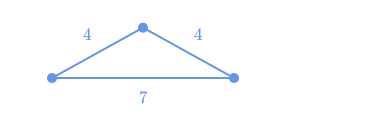
\includegraphics[scale=\shrinkfactor]{figures/a5961a517a4e6e5e6def530e3948dc049dbfad9a.png}

\paragraph{Hint 3}Given the conditions, only one triangle can be drawn.



\medskip
\noindent
\textbf{Tags:} {\footnotesize Constructing triangles, CC.7.G.A.2}\\
\textbf{Version:} 7bc13eed.. 2013-10-21
\smallskip\hrule





\section{\href{https://www.khanacademy.org/devadmin/content/items/x38cc51ab93842600}{x38cc51ab93842600}}

\noindent
**How many triangles can be drawn with side lengths $1$, $1$ and $2.5$?**

\paragraph{Ans} 

\fbox{ None

}

 Only one

More than one



\paragraph{Hint 1}A triangle is a plane figure with three straight sides and three angles. Can we satisfy the definition given the conditions? Let's try to draw a triangle given the conditions.

\paragraph{Hint 2}In general, any side of a triangle is always shorter than the sum of the other two sides. Because $\blue{2.5} >\blue{1}+\blue{1}$, the two sides $\blue{1}$ and $\blue{1}$ cannot meet to form a third angle over the third side $\blue{2.5}$. 


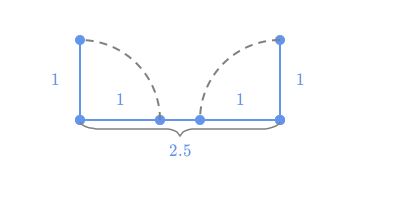
\includegraphics[scale=\shrinkfactor]{figures/cb4884edd39739116b62d131aa206b66f99db2cb.png}

We cannot create three angles to satisfy the definition of a triangle.

\paragraph{Hint 3}Given the conditions, no triangles can be drawn.



\medskip
\noindent
\textbf{Tags:} {\footnotesize Constructing triangles, CC.7.G.A.2}\\
\textbf{Version:} 05f2acc5.. 2013-10-21
\smallskip\hrule





\section{\href{https://www.khanacademy.org/devadmin/content/items/x4c335bfbee0cba92}{x4c335bfbee0cba92}}

\noindent
**Draw a right triangle with at least two sides of equal length.** 

**Is there a unique triangle that satisfies the given conditions?**
[[? interactive-graph 1]]

\paragraph{Ans} 

Yes

\fbox{ No

}

 

\paragraph{Hint 1}Let�s start by drawing. A right triangle has one $\blue{90 ^\circ}$ angle. 

A triangle with at least two equal side lengths is called an isosceles triangle. We do not know the side lengths.

\paragraph{Hint 2}We can draw many right triangles with two sides of  equal length.  

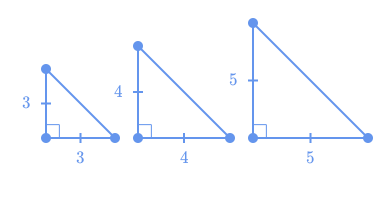
\includegraphics[scale=\shrinkfactor]{figures/d8b2dd5b2d43266692ba3d2c35cf5638f2f3c05c.png}

\paragraph{Hint 3}The triangle is not unique.



\medskip
\noindent
\textbf{Tags:} {\footnotesize Constructing triangles, CC.7.G.A.2}\\
\textbf{Version:} 381a8a90.. 2013-10-21
\smallskip\hrule





\section{\href{https://www.khanacademy.org/devadmin/content/items/x531e157ba7c498eb}{x531e157ba7c498eb}}

\noindent
**How many triangles can be drawn where the measures of all three angles are the same?**

\paragraph{Ans} 

None

Only one

\fbox{ More than one

}

 

\paragraph{Hint 1}A triangle is a plane figure with three straight sides and three angles. What triangle or triangles would satisfy the conditions? 

Let's try to draw a triangle where the measures of all three angles is the same. 

\paragraph{Hint 2}The three angle measures in a triangle must sum to $\pink{180^\circ}$. Because we know the measure of all three angles must be the same, we know all three angles have measure $\dfrac{\pink{180^\circ}}{3}=\blue{60^\circ}$. 


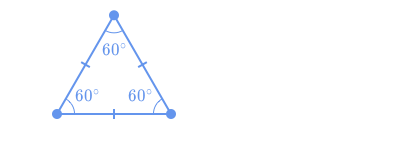
\includegraphics[scale=\shrinkfactor]{figures/9bbd0fa30a5ae16d50c816c4a8c4cfc44a68146c.png}

This is an equilateral triangle.


\paragraph{Hint 3}Is this triangle unique or do other equilateral triangles exist with a different size?

We can draw many equilateral triangles with the same shape but different sizes.


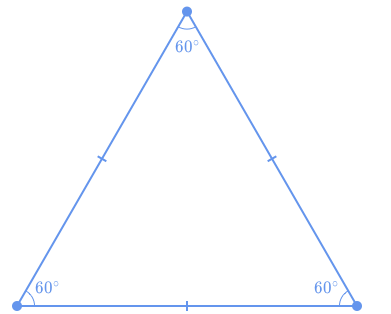
\includegraphics[scale=\shrinkfactor]{figures/3e0462daa95058cdd7264a43f9c163723c418fd6.png}

\paragraph{Hint 4}More than one triangle can be drawn with all three angles measures equal.



\medskip
\noindent
\textbf{Tags:} {\footnotesize Constructing triangles, CC.7.G.A.2}\\
\textbf{Version:} 1ab79063.. 2013-10-21
\smallskip\hrule





\section{\href{https://www.khanacademy.org/devadmin/content/items/x572fecbc70b353aa}{x572fecbc70b353aa}}

\noindent
**Draw a right triangle that is also an isosceles triangle and has two sides of length $3$.** 

**Is there a unique triangle that satisfies the given conditions?**   
[[? interactive-graph 1]]

\paragraph{Ans} 

\fbox{ Yes

}

 No



\paragraph{Hint 1}Let�s start by drawing. A right triangle has one $\blue{90^\circ}$ angle. 

An isosceles triangle has at least two side lengths equal. We are given two side lengths both equal to $\blue3$. 

\paragraph{Hint 2}Let's draw one side length $\blue{3}$ as the height vertically (up and down) from the $\blue{90 ^\circ}$ angle. Let's draw the other side length $\blue{3}$ as the base horizontally (left and right) from the $\blue{90^\circ}$ angle. 

\paragraph{Hint 3}Since we are given the measures of two sides and the angle between them, we can draw only one triangle.

\paragraph{Hint 4}The triangle is unique.

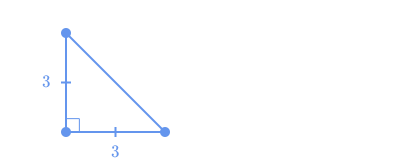
\includegraphics[scale=\shrinkfactor]{figures/29740936508e0ec4c2d3167e2aec0f3372ce78bf.png}



\medskip
\noindent
\textbf{Tags:} {\footnotesize Constructing triangles, CC.7.G.A.2}\\
\textbf{Version:} 42221dd1.. 2013-10-21
\smallskip\hrule





\section{\href{https://www.khanacademy.org/devadmin/content/items/x651844ecfaac48e9}{x651844ecfaac48e9}}

\noindent
**Draw a right triangle with two $45^\circ$ angles.**

**Is there a unique triangle that satisfies the given conditions?**
[[? interactive-graph 1]]

\paragraph{Ans} 

Yes

\fbox{ No

}

 

\paragraph{Hint 1}Let�s start by drawing. A right triangle has one $\blue{90^\circ}$ angle. 

The triangle we want is an isosceles right triangle. An isosceles right triangle has two $\blue{45^\circ}$ angles.

\paragraph{Hint 2}We know the measure of all three angles but not the length of any side. Therefore, we can draw many triangles of various sizes all with a pair of $\blue{45^\circ}$ angles.


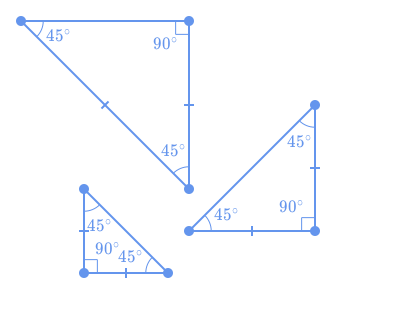
\includegraphics[scale=\shrinkfactor]{figures/91996cb5320f958d2fa0f8249c77e9d88bbb2764.png}


\paragraph{Hint 3}The triangle is not unique.




\medskip
\noindent
\textbf{Tags:} {\footnotesize Constructing triangles, CC.7.G.A.2}\\
\textbf{Version:} fb842816.. 2013-10-21
\smallskip\hrule





\section{\href{https://www.khanacademy.org/devadmin/content/items/x6763ceb1ec0ceb41}{x6763ceb1ec0ceb41}}

\noindent
**How many triangles can be drawn where the lengths of all three sides are equal to $1$?**

\paragraph{Ans} 

None

\fbox{ Only one

}

 More than one



\paragraph{Hint 1}A triangle is a plane figure with three straight sides and three angles. Is there a triangle or triangles that satisfy the conditions? Let's try to draw a triangle with all side lengths equal to $\blue1$.

\paragraph{Hint 2}The result is an equilateral triangle with equal side lengths and equal angles measures:


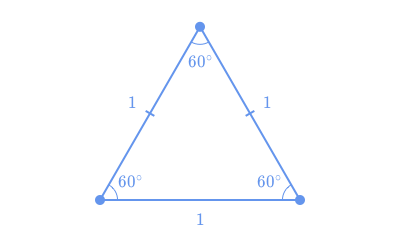
\includegraphics[scale=\shrinkfactor]{figures/b0e7ebe35f997eac2f27bbad47f0033422d118b3.png}

This triangle is unique, meaning no other triangle exists that has all sides equal to $\blue1$.

\paragraph{Hint 3}In general, if the lengths of all three sides are known, only one triangle can be drawn.



\medskip
\noindent
\textbf{Tags:} {\footnotesize Constructing triangles, CC.7.G.A.2}\\
\textbf{Version:} e412934c.. 2013-10-21
\smallskip\hrule





\section{\href{https://www.khanacademy.org/devadmin/content/items/x67ee6010588311f2}{x67ee6010588311f2}}

\noindent
**How many triangles can be drawn with side lengths $4$, $6$ and $11$?**

\paragraph{Ans} 

\fbox{ None

}

 Only one

More than one



\paragraph{Hint 1}A triangle is a plane figure with three straight sides and three angles. Can we satisfy the definition given the conditions? Let's try to draw a triangle given the conditions.

\paragraph{Hint 2}In general, any side of a triangle is always shorter than the sum of the other two sides. Because $\blue{11} >\blue{6}+\blue{4}$, the two sides $\blue{6}$ and $\blue{4}$ cannot meet to form a third angle over the third side $\blue{11}$. 


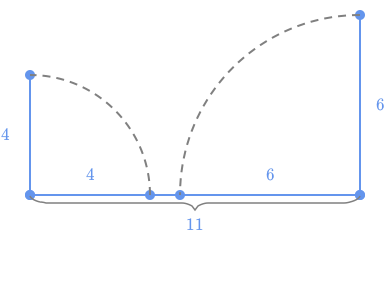
\includegraphics[scale=\shrinkfactor]{figures/6b60caa69910861ed0aa6e21b79d5cde304168b3.png}

We cannot create three angles to satisfy the definition of a triangle.

\paragraph{Hint 3}Given the conditions, no triangles can be drawn.



\medskip
\noindent
\textbf{Tags:} {\footnotesize Constructing triangles, CC.7.G.A.2}\\
\textbf{Version:} edcac7f5.. 2013-10-21
\smallskip\hrule





\section{\href{https://www.khanacademy.org/devadmin/content/items/x67fd10caf4f54df2}{x67fd10caf4f54df2}}

\noindent
**Draw a right triangle with side lengths $3a$,  $4a$ and $5a$, where $a$ is any positive number.**

**Is there a unique triangle that satisfies the given conditions?**
[[? interactive-graph 1]]

\paragraph{Ans} 

Yes

\fbox{ No

}

 

\paragraph{Hint 1}Let�s start by choosing a value for $\pink{a}$ where $\pink{a}$ is any positive number, then we can draw a right triangle with side lengths $\purple3\pink{a}$, $\purple4\pink{a}$ and $\purple5\pink{a}$.

\paragraph{Hint 2}If $\pink{a}=1$, then we can draw a right triangle with side lengths $\blue3$, $\blue4$ and $\blue5$. 

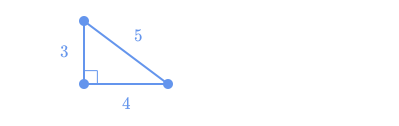
\includegraphics[scale=\shrinkfactor]{figures/b1eff2246ff6077c50f40ea6bfe55bad4b8ced80.png}

\paragraph{Hint 3}If $\pink{a}=2$, then we can draw a right triangle with side lengths $\blue6$, $\blue8$ and $\blue{10}$. 

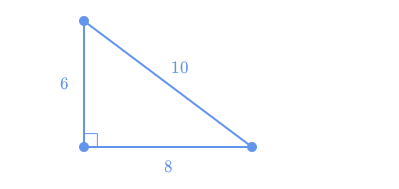
\includegraphics[scale=\shrinkfactor]{figures/ef5a8edbd9d4f5680b124ce81e7f4c78a9707ed4.png}

We can let $\pink{a}$ be any positive number and draw many triangles of same shape but different sizes.

\paragraph{Hint 4}The triangle is not unique. Multiple triangles satisfy the conditions.


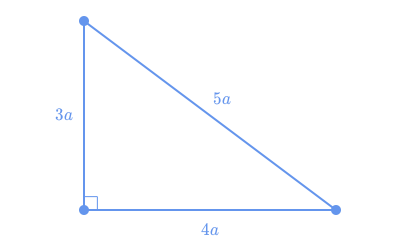
\includegraphics[scale=\shrinkfactor]{figures/946760cec54502326e2f2708bb7c84428118c9ad.png}



\medskip
\noindent
\textbf{Tags:} {\footnotesize Constructing triangles, CC.7.G.A.2}\\
\textbf{Version:} 0b713fdb.. 2013-10-21
\smallskip\hrule





\section{\href{https://www.khanacademy.org/devadmin/content/items/x6d7be6276bcb5815}{x6d7be6276bcb5815}}

\noindent
**Draw a right triangle with a height $4$ and base  $5$.** 

**Is there a unique triangle that satisfies the given conditions?**
[[? interactive-graph 1]]

\paragraph{Ans} 

\fbox{ Yes

}

 No



\paragraph{Hint 1}Let�s start by drawing. A right triangle has a $\blue{90^\circ}$ angle. 

The height of length $\blue{4}$ is drawn vertically (up and down) from the $\blue{90^\circ}$ angle. The base of length $\blue{5}$ is drawn horizontally (left and right) from the $\blue{90^\circ}$ angle. 

\paragraph{Hint 2}Since we are given the measures of two sides and the angle between them, we can draw only one triangle.

\paragraph{Hint 3}The triangle is unique.


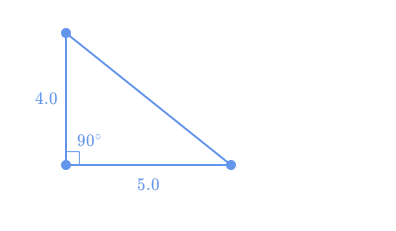
\includegraphics[scale=\shrinkfactor]{figures/21924a4df5c1451289595e8ec2c9ceae30ed7de1.png}



\medskip
\noindent
\textbf{Tags:} {\footnotesize Constructing triangles, CC.7.G.A.2}\\
\textbf{Version:} 77539544.. 2013-10-21
\smallskip\hrule





\section{\href{https://www.khanacademy.org/devadmin/content/items/x72d893d1e3229dfd}{x72d893d1e3229dfd}}

\noindent
**How many triangles can we draw with side lengths  $3$ and $4$?**

\paragraph{Ans} 

None

Only one

\fbox{ More than one

}

 

\paragraph{Hint 1}We can  draw many triangles with side lengths $\blue3$ and $\blue{4}$.


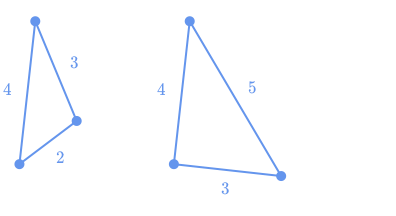
\includegraphics[scale=\shrinkfactor]{figures/2d99bebb2da26f68f4d74679d523ed8d96db3e5c.png}

\paragraph{Hint 2}Without knowing at least one angle measure, we cannot create a unique triangle with side lengths $\blue3$ and $\blue4$.

\paragraph{Hint 3}If we only know two side lengths, more than one triangle can be drawn.



\medskip
\noindent
\textbf{Tags:} {\footnotesize Constructing triangles, CC.7.G.A.2}\\
\textbf{Version:} 7f5a7177.. 2013-10-21
\smallskip\hrule





\section{\href{https://www.khanacademy.org/devadmin/content/items/x892857b71e427c39}{x892857b71e427c39}}

\noindent
**How many triangles can be drawn with angles $60^\circ$,  $60^\circ$ and $70^\circ$?**

\paragraph{Ans} 

\fbox{ None

}

 Only one

More than one



\paragraph{Hint 1}A triangle is a plane figure with three straight sides and three angles. In a triangle, the sum of the three angle measures is $\pink{180^\circ}$.

\paragraph{Hint 2}Let's add together the angles measures $\blue{60}^\circ$,  $\blue{60}^\circ$ and $\blue{70}^\circ$:

\begin{align*} 
\text{sum of angle measures} 
&= \blue{60^\circ} + \blue{60^\circ}+\blue{70^\circ}\\
&= 120^\circ+70^\circ\\
&= 190^\circ\\
\end{align*}

The sum of the three angle measures is greater than $\pink{180^\circ}$.

\paragraph{Hint 3}No triangle can be drawn that satisfies the given conditions.



\medskip
\noindent
\textbf{Tags:} {\footnotesize Constructing triangles, CC.7.G.A.2}\\
\textbf{Version:} b659944d.. 2013-10-21
\smallskip\hrule





\section{\href{https://www.khanacademy.org/devadmin/content/items/xb880da8414b8f195}{xb880da8414b8f195}}

\noindent
**Draw an obtuse triangle with angles $45^\circ$,  $35^\circ$ and $100^\circ$.**

**Is there a unique triangle that satisfies the given conditions?**
[[? interactive-graph 1]]

\paragraph{Ans} 

Yes

\fbox{ No

}

 

\paragraph{Hint 1}Let�s start by drawing. While keeping one angle constant, we can change the side lengths to create one of the other two angles.

For example, while keeping a $\blue{45^\circ}$ angle, we can change the side lengths to create the $\blue{35^\circ}$ angle. The third angle will have measure $\blue{100^\circ}$.

\paragraph{Hint 2}We know the measure of three angles but not the length of any side. We can draw many triangles of same shape but different sizes.

\paragraph{Hint 3}The triangle is not unique.


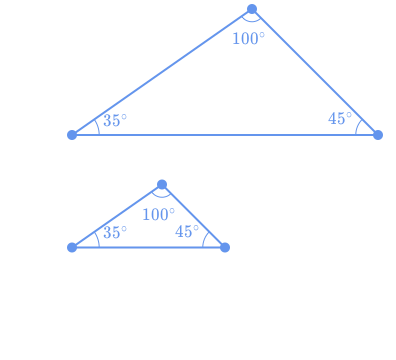
\includegraphics[scale=\shrinkfactor]{figures/c6b48cf353062cc42130d16552b68f58a6daf58e.png}



\medskip
\noindent
\textbf{Tags:} {\footnotesize Constructing triangles, CC.7.G.A.2}\\
\textbf{Version:} 6879cae0.. 2013-10-21
\smallskip\hrule





\section{\href{https://www.khanacademy.org/devadmin/content/items/xb9aa47b3de982d55}{xb9aa47b3de982d55}}

\noindent
**Draw an isosceles triangle with two $70^\circ$ angles.**

**Is there a unique triangle that satisfies the given conditions?**
[[? interactive-graph 1]]

\paragraph{Ans} 

Yes

\fbox{ No

}

 

\paragraph{Hint 1}Let�s start by drawing an isosceles triangle with two $\blue{70^\circ}$ angles. An isosceles triangle has at least two side lengths equal and two angles equal.

\paragraph{Hint 2}We do not know the side lengths, so we can draw many triangles.

\paragraph{Hint 3}The triangle is not unique.

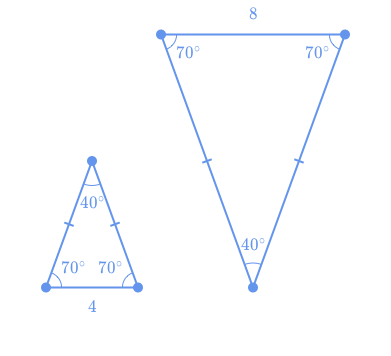
\includegraphics[scale=\shrinkfactor]{figures/afb29f0a848d89c4b6991b76cd2f1a48e594243b.png}



\medskip
\noindent
\textbf{Tags:} {\footnotesize Constructing triangles, CC.7.G.A.2}\\
\textbf{Version:} c30a9e63.. 2013-10-21
\smallskip\hrule





\section{\href{https://www.khanacademy.org/devadmin/content/items/xbd061a8700fced6c}{xbd061a8700fced6c}}

\noindent
**How many right triangles can be drawn with angles $40^\circ$ and  $60^\circ$?**

\paragraph{Ans} 

\fbox{ None

}

 Only one

More than one



\paragraph{Hint 1}A triangle is a plane figure with three straight sides and three angles. In a triangle, the sum of the three angle measures is $\pink{180^\circ}$.

A right triangle has a $\blue{90}^\circ$  angle.

\paragraph{Hint 2}Let's add together the angle measures $\blue{40}^\circ$,  $\blue{60}^\circ$ and $\blue{90}^\circ$:

\begin{align*}
\text{sum of angle measures} 
 &=  \blue{40^\circ}+\blue{60^\circ}+\blue{90^\circ}\\
&= 190^\circ\end{align*}

The sum of the three angles is greater than $\pink{180^\circ}$.

\paragraph{Hint 3}No triangle can be drawn that satisfies the given conditions.



\medskip
\noindent
\textbf{Tags:} {\footnotesize Constructing triangles, CC.7.G.A.2}\\
\textbf{Version:} 24dc4864.. 2013-10-21
\smallskip\hrule





\section{\href{https://www.khanacademy.org/devadmin/content/items/xc001c788d01d9e5f}{xc001c788d01d9e5f}}

\noindent
**Draw a triangle with two angles $58^\circ$ and $90^\circ$ where side length $4$ is *not* between the two angles $58^\circ$ and $90^\circ$.**

**Is there a unique triangle that satisfies the given conditions?**
[[? interactive-graph 1]]

\paragraph{Ans} 

\fbox{ Yes

}

 No



\paragraph{Hint 1}Let�s start by drawing a right angle which is $\blue{90^\circ}$. 

Then, let's draw the side of length $\blue4$ next to the right angle, so our base has a length of $\blue4$.

\paragraph{Hint 2}The side of length $\blue4$ is $\red{\text{not}}$ between two angles $\blue{58^\circ}$ and $\blue{90^\circ}$. 

Since we drew the side of length $\blue4$ next to the right angle, the $\blue{58^\circ}$ angle must be *opposite* the side of length $\blue4$ .

\paragraph{Hint 3}We know the measure of two angles and the length of one side not between the angles, so we can draw only one triangle.

\paragraph{Hint 4}The triangle is unique.


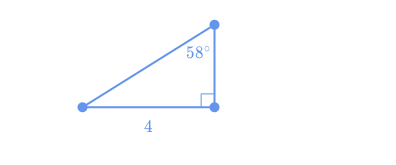
\includegraphics[scale=\shrinkfactor]{figures/0ddd88656709215709e4a46913277db7929349d4.png}



\medskip
\noindent
\textbf{Tags:} {\footnotesize Constructing triangles, CC.7.G.A.2}\\
\textbf{Version:} c15babbe.. 2013-10-21
\smallskip\hrule





\section{\href{https://www.khanacademy.org/devadmin/content/items/xc256611ab7d92e83}{xc256611ab7d92e83}}

\noindent
**Draw a triangle with side length $5$ between two $58^\circ$ angles.** 

**Is there a unique triangle that satisfies the given conditions?**
[[? interactive-graph 1]]

\paragraph{Ans} 

\fbox{ Yes

}

 No



\paragraph{Hint 1}Let�s start by drawing the length of one side, which we know is $\blue5$.  

\paragraph{Hint 2}From the side $\blue5$, let�s draw two $\blue{58^\circ}$ angles. Since we have two equal angles, we have an isosceles triangle. An isosceles triangle has at least two sides equal in length. 

Since we have two $\blue{58^\circ}$ angles, the third angle must be $\green{64^\circ}$. The sum of  three angles in a triangle will always be $\pink{180^\circ}$.

\paragraph{Hint 3}We know the measure of two angles and the length of the side between the angles, so we can draw only one triangle.

\paragraph{Hint 4}The triangle is unique.


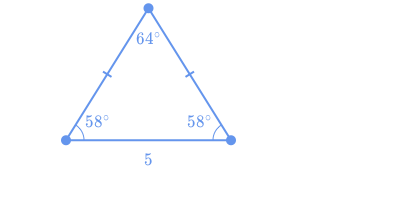
\includegraphics[scale=\shrinkfactor]{figures/4af5c292b250f14e2725fbff73825f6e41348a27.png}



\medskip
\noindent
\textbf{Tags:} {\footnotesize Constructing triangles, CC.7.G.A.2}\\
\textbf{Version:} 7d6f4977.. 2013-10-21
\smallskip\hrule





\section{\href{https://www.khanacademy.org/devadmin/content/items/xc40b1278855716df}{xc40b1278855716df}}

\noindent
**Draw a right triangle with side lengths $3$, $4$ and $5$.** 

**Is there a unique triangle that satisfies the given conditions?**
[[? interactive-graph 1]]

\paragraph{Ans} 

\fbox{ Yes

}

 No



\paragraph{Hint 1}Let�s start by drawing. We know the lengths of all three sides. How many triangles can we draw?

\paragraph{Hint 2}The triangle with side lengths $\blue3$, $\blue4$ and $\blue5$ is a right triangle. Since we are given the measures of three sides, we can draw only one triangle. 

\paragraph{Hint 3}The triangle is unique.


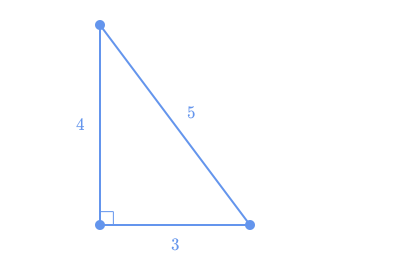
\includegraphics[scale=\shrinkfactor]{figures/758d66a2a3006feaf0b6d196067ab8a9e5a4c587.png}



\medskip
\noindent
\textbf{Tags:} {\footnotesize Constructing triangles, CC.7.G.A.2}\\
\textbf{Version:} 3adc68e6.. 2013-10-21
\smallskip\hrule





\section{\href{https://www.khanacademy.org/devadmin/content/items/xdba9a2b900c8bbcd}{xdba9a2b900c8bbcd}}

\noindent
**How many triangles can be drawn with side lengths $1$, $2$ and $4$?**

\paragraph{Ans} 

\fbox{ None

}

 Only one

More than one



\paragraph{Hint 1}A triangle is a plane figure with three straight sides and three angles. Can we satisfy the definition given the conditions? Let's try to draw a triangle given the conditions.

\paragraph{Hint 2}In general, any side of a triangle is always shorter than the sum of the other two sides. Because $\blue{4} >\blue{2}+\blue{1}$, the two sides $\blue{2}$ and $\blue{1}$ cannot meet to form a third angle over the third side $\blue{4}$. 


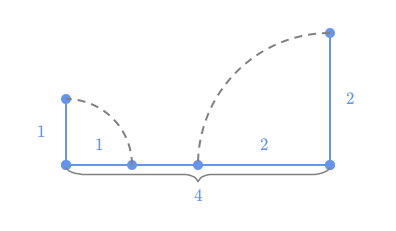
\includegraphics[scale=\shrinkfactor]{figures/dbd401421f460f804da516fa3a58107492fea141.png}

We cannot create three angles to satisfy the definition of a triangle.

\paragraph{Hint 3}Given the conditions, no triangles can be drawn.



\medskip
\noindent
\textbf{Tags:} {\footnotesize Constructing triangles, CC.7.G.A.2}\\
\textbf{Version:} 950a8286.. 2013-10-21
\smallskip\hrule





\section{\href{https://www.khanacademy.org/devadmin/content/items/xe06107bc78ca0b3c}{xe06107bc78ca0b3c}}

\noindent
**How many triangles can we draw with angles $30^\circ$,  $50^\circ$ and $100^\circ$?**

\paragraph{Ans} 

None

Only one

\fbox{ More than one

}

 

\paragraph{Hint 1}A triangle is a plane figure with three straight sides and three angles. The three angles measures must add up to $\pink{180^\circ}$. Let's add together the angles $\blue{30}^\circ$,  $\blue{50}^\circ$ and $\blue{100}^\circ$:

\begin{align*} 
\text{total angle measure} &= \blue{30^\circ}+\blue{50^\circ}+\blue{180^\circ}\\
&=\pink{180^\circ}
\end{align*}

So, at least one triangle exists. Let's draw.

\paragraph{Hint 2}We know the measure of three angles but not the length of any side. We can draw many triangles with the same shape but different sizes.


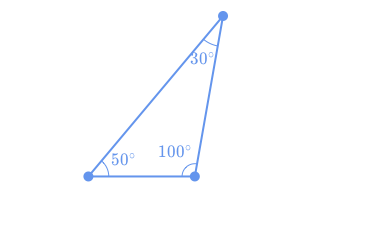
\includegraphics[scale=\shrinkfactor]{figures/cfa8c2afddab68081b192038f3130d47880b443e.png}

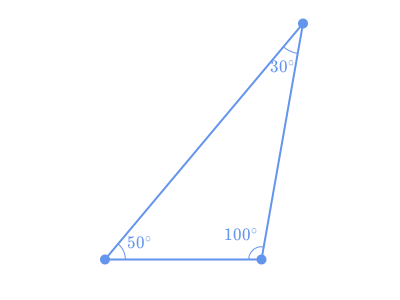
\includegraphics[scale=\shrinkfactor]{figures/b1683148f0f59becb3f7ee5221cd130e632609d7.png}

\paragraph{Hint 3}When only the measures of all three angles are known, more than one triangle can be drawn.



\medskip
\noindent
\textbf{Tags:} {\footnotesize Constructing triangles, CC.7.G.A.2}\\
\textbf{Version:} 7c205db7.. 2013-10-21
\smallskip\hrule





\section{\href{https://www.khanacademy.org/devadmin/content/items/xe937d430ba8d75d8}{xe937d430ba8d75d8}}

\noindent
**How many triangles can we draw that have one angle measure equal to $45^\circ$ and one side of length $5$?**

\paragraph{Ans} 

None

Only one

\fbox{ More than one

}

 

\paragraph{Hint 1}A triangle is a plane figure with three straight sides and three angles. 

The three angles measures always add up to $\pink{180^\circ}$. We only know one angle is $\blue{45^\circ}$. We can't find the measures of the other two angles.

\paragraph{Hint 2}We know the length of only one side is $\blue5$. Depending if we place the side of length $\blue5$ next to or across from the $\blue{45^\circ}$ angle, we can  draw many triangles with different shapes and different sizes.


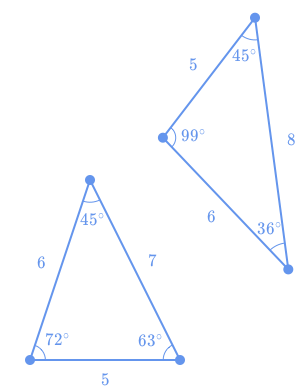
\includegraphics[scale=\shrinkfactor]{figures/8fd2ab6db3cbbe9cbdf43af4cf872835fa89ecf2.png}

\paragraph{Hint 3}If we only know one angle and one side length, more than one triangle can be drawn.



\medskip
\noindent
\textbf{Tags:} {\footnotesize Constructing triangles, CC.7.G.A.2}\\
\textbf{Version:} e1956610.. 2013-10-21
\smallskip\hrule





\section{\href{https://www.khanacademy.org/devadmin/content/items/xf51994a651ca1d7f}{xf51994a651ca1d7f}}

\noindent
**Draw a triangle with angles $30^\circ$,  $50^\circ$ and $100^\circ$.**

**Is there a unique triangle that satisfies the given conditions?**
[[? interactive-graph 1]]

\paragraph{Ans} 

Yes

\fbox{ No

}

 

\paragraph{Hint 1}Let�s start by drawing. While keeping one angle, we can change the side lengths to create one of the other two angles.

While keeping a $\blue{100^\circ}$ angle, we can change the side lengths to create the $\blue{50^\circ}$ angle. The final angle will be $\blue{30^\circ}$.

\paragraph{Hint 2}We know the measure of three angles but not the length of any side. We can draw many triangles of same shape but different sizes.

\paragraph{Hint 3}The triangle is not unique.

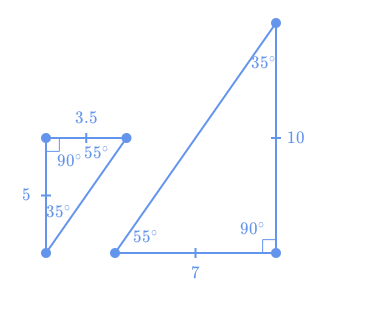
\includegraphics[scale=\shrinkfactor]{figures/13ed90e8845185b7c961687bdf49c22135f67ec5.png}



\medskip
\noindent
\textbf{Tags:} {\footnotesize Constructing triangles, CC.7.G.A.2}\\
\textbf{Version:} d7e4aa43.. 2013-10-21
\smallskip\hrule





\section{\href{https://www.khanacademy.org/devadmin/content/items/xf9872931929ac56c}{xf9872931929ac56c}}

\noindent
**Draw a right triangle with side lengths $5$, $12$ and $13$.** 

**Is there a unique triangle that satisfies the given conditions?**
[[? interactive-graph 1]]

\paragraph{Ans} 

\fbox{ Yes

}

 No



\paragraph{Hint 1}Let�s start by drawing. We know the lengths of all three sides. How many right triangles can we draw?

\paragraph{Hint 2}Since we are given the lengths of all three sides, we can draw only one right triangle with side lengths $\blue5$, $\blue{12}$ and $\blue{13}$.


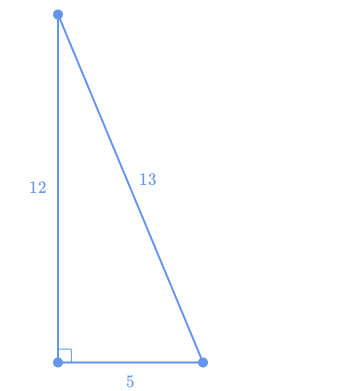
\includegraphics[scale=\shrinkfactor]{figures/227ab289b1de518857460dab83b70e050be9fa46.png}

\paragraph{Hint 3}The triangle is unique.



\medskip
\noindent
\textbf{Tags:} {\footnotesize Constructing triangles, CC.7.G.A.2}\\
\textbf{Version:} ba30b682.. 2013-10-21
\smallskip\hrule



%%  Create a directory called 'figures' in latex dir and run the following command 
%  wget -N \
%    https://ka-perseus-graphie.s3.amazonaws.com/8664b06c420b8bf33711310103a6963e0f2cc7f1.png \
%    https://ka-perseus-graphie.s3.amazonaws.com/9e3335e4646b2e59f3ceb8860cd9099de97f22b0.png \
%    https://ka-perseus-graphie.s3.amazonaws.com/6d298ed14c507f692b6d88792d963d7008b9847a.png \
%    https://ka-perseus-graphie.s3.amazonaws.com/463955e595c31361c49d853aea12289b0f5f7779.png \
%    https://ka-perseus-graphie.s3.amazonaws.com/28bab6f73b266fa0cb6392a48f06caca532f0cd2.png \
%    https://ka-perseus-graphie.s3.amazonaws.com/42e1efd00be59b64d19c796b09c66213066bd2fa.png \
%    https://ka-perseus-graphie.s3.amazonaws.com/fe9bb66c73daee381242a48159a578e8b78ac0fb.png \
%    https://ka-perseus-graphie.s3.amazonaws.com/50ab52075216ec1ebe030aa80de8615558c71846.png \
%    https://ka-perseus-graphie.s3.amazonaws.com/48773248b446b970cdf6c2fa7664c3fa8890378a.png \
%    https://ka-perseus-graphie.s3.amazonaws.com/a5961a517a4e6e5e6def530e3948dc049dbfad9a.png \
%    https://ka-perseus-graphie.s3.amazonaws.com/cb4884edd39739116b62d131aa206b66f99db2cb.png \
%    https://ka-perseus-graphie.s3.amazonaws.com/d8b2dd5b2d43266692ba3d2c35cf5638f2f3c05c.png \
%    https://ka-perseus-graphie.s3.amazonaws.com/9bbd0fa30a5ae16d50c816c4a8c4cfc44a68146c.png \
%    https://ka-perseus-graphie.s3.amazonaws.com/3e0462daa95058cdd7264a43f9c163723c418fd6.png \
%    https://ka-perseus-graphie.s3.amazonaws.com/29740936508e0ec4c2d3167e2aec0f3372ce78bf.png \
%    https://ka-perseus-graphie.s3.amazonaws.com/91996cb5320f958d2fa0f8249c77e9d88bbb2764.png \
%    https://ka-perseus-graphie.s3.amazonaws.com/b0e7ebe35f997eac2f27bbad47f0033422d118b3.png \
%    https://ka-perseus-graphie.s3.amazonaws.com/6b60caa69910861ed0aa6e21b79d5cde304168b3.png \
%    https://ka-perseus-graphie.s3.amazonaws.com/b1eff2246ff6077c50f40ea6bfe55bad4b8ced80.png \
%    https://ka-perseus-graphie.s3.amazonaws.com/ef5a8edbd9d4f5680b124ce81e7f4c78a9707ed4.png \
%    https://ka-perseus-graphie.s3.amazonaws.com/946760cec54502326e2f2708bb7c84428118c9ad.png \
%    https://ka-perseus-graphie.s3.amazonaws.com/21924a4df5c1451289595e8ec2c9ceae30ed7de1.png \
%    https://ka-perseus-graphie.s3.amazonaws.com/2d99bebb2da26f68f4d74679d523ed8d96db3e5c.png \
%    https://ka-perseus-graphie.s3.amazonaws.com/c6b48cf353062cc42130d16552b68f58a6daf58e.png \
%    https://ka-perseus-graphie.s3.amazonaws.com/afb29f0a848d89c4b6991b76cd2f1a48e594243b.png \
%    https://ka-perseus-graphie.s3.amazonaws.com/0ddd88656709215709e4a46913277db7929349d4.png \
%    https://ka-perseus-graphie.s3.amazonaws.com/4af5c292b250f14e2725fbff73825f6e41348a27.png \
%    https://ka-perseus-graphie.s3.amazonaws.com/758d66a2a3006feaf0b6d196067ab8a9e5a4c587.png \
%    https://ka-perseus-graphie.s3.amazonaws.com/dbd401421f460f804da516fa3a58107492fea141.png \
%    https://ka-perseus-graphie.s3.amazonaws.com/cfa8c2afddab68081b192038f3130d47880b443e.png \
%    https://ka-perseus-graphie.s3.amazonaws.com/b1683148f0f59becb3f7ee5221cd130e632609d7.png \
%    https://ka-perseus-graphie.s3.amazonaws.com/8fd2ab6db3cbbe9cbdf43af4cf872835fa89ecf2.png \
%    https://ka-perseus-graphie.s3.amazonaws.com/13ed90e8845185b7c961687bdf49c22135f67ec5.png \
%    https://ka-perseus-graphie.s3.amazonaws.com/227ab289b1de518857460dab83b70e050be9fa46.png \


\end{document}
